\chapter{Programmets brugergrænseflade}



I dette kapitel vil programmet grafiske brugergrænseflade blive beskrevet.


% LaTeX tabel som viser alle brugerniveauer og deres muligheder efter login.
% http://bit.ly/1kToHZ3 to edit raw table
\begin{table}
    \colorlet{shadecolor}{gray!40}
    \rowcolors{1}{white}{shadecolor}
    \begin{tabular}{l|llllll}
    ~                        & Gæst & Støttemedlem & Medlem & Elev & Underviser & Administrator \\ \hline
    Personlig forside        & ~    & ~             & \ding{51}     & \ding{51}    & \ding{51}          & \ding{51}             \\
    Se begivenheder          & \ding{51}    & \ding{51}             & \ding{51}      & \ding{51}    & \ding{51}          & \ding{51}             \\
    Tilmeld begivenheder     & ~    & ~	             & \ding{51}      & \ding{51}    & \ding{51}          & \ding{51}             \\
    Opret begivenheder       & ~    & ~             & ~      & ~    & \ding{51}          & \ding{51}             \\
    Se sejlture              & \ding{51}    & \ding{51}             & \ding{51}      & \ding{51}    & \ding{51}          & \ding{51}             \\
    Opret sejltur            & ~    & ~             & \ding{51}      & \ding{51}    & \ding{51}          & \ding{51}             \\
    Se logbøger              & \ding{51}    & \ding{51}             & \ding{51}      & \ding{51}    & \ding{51}          & \ding{51}             \\
    Opret logbog             & ~    & ~             & \ding{51}      & \ding{51}    & \ding{51}          & \ding{51}             \\
    Svar på logbog           & ~    & ~             & ~      & ~    & ~          & \ding{51}             \\
    Se undervisningstimer    & ~    & ~             & ~      & \ding{51}    & \ding{51}          & \ding{51}             \\
    Opret undervisningstimer & ~    & ~             & ~      & ~    & \ding{51}          & \ding{51}             \\
    \end{tabular}
    \caption{Tabel over alle brugerniveauer og deres tilladte funktioner.}\label{tab:permissions}\fixme{Måske skal denne tabel lige laves lidt om, enten indholdet, eller hvordan det virker i programmet.}
\end{table}

\section{Hovedvinduet}
Hovedvinduet tilgås via loginvinduet, som starter ved programstart eller ved at trykke på logudknappen inde fra hovedvinduet selv. 
Der findes fire udgaver af hovedvinduet, forskellen mellem dem er, hvilke tabs der er aktive.
Hver tab indeholder forskellige funktioner, samlet set findes følgende tabs:
\begin{itemize}% Denne skulle måske relatere til tabel tab:permission
    \item Forside
    \item Undervisning
    \item Begivenheder
    \item Medlemmer
    \item Både
\end{itemize}

Via hver af disse tabs, vil der være adgang til programmets forskellige funktionaliteter.
Der er også en logud knap, som bruges til at vende tilbage til loginvinduet, således en anden bruger kan anvende systemet.
Programmet er lavet til at køre i opløsningen 1024x720 pixels.
Denne opløsning er valgt for at understøtte alt fra bærbare, med opløsninger som 1366x768 pixels i et vindue, og op til FullHD (1920x1080 pixels) op op efter. 
Stort set alle computerskærme har en opløsning større end 1024x720 pixels\citep{resolutions}. 
Programmet har et lyst farveskema; med farverne hvid og en lys blå som hovedfarver (\#87D4EE).

\section{UserControls}
Der anvendes Usercontrols til at kode både brugergrænsefladen og den tilhørende Code-Behind.

\subsection{DateTimePicker}\label{subsec:DateTimePicker}

\begin{wrapfigure}{r}{0.5\textwidth}
    \label{img:DateTimePicker}
    \vspace{-20pt}
    \begin{center}
        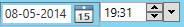
\includegraphics[width=0.48\textwidth]{Screenshots/DateTimePicker.png}
    \end{center}
    \vspace{-15pt}
    \caption{DateTimePicker}
    \vspace{-30pt}
\end{wrapfigure}

\textbf{Formål}: 
Denne Usercontrol er lavet, da der ikke fandtes en tilfredsstillende løsning, som gjorde det muligt at vælge både dato og tidspunkt i samme control. 
Det er ofte nødvendigt at vælge både dato og tidspunkt samtidigt. 

\textbf{BrugerGrænseflade}: 
Den består af en DatePicker, og en TimePicker som findes i extended WPF toolkit.

\textbf{Code-Behind}: 
Der er blevet lavet en specialfremstillet getter og setter for Usercontrolen. 


\subsection{Forside}

\textbf{Formål}: 
Formålet med forsiden er at vise aktuel infomation på en overskuelig måde for brugeren.
Det er den første side i hovedvinduet, som man ser, med mindre man er gæst.
Fra forsiden kan man ændre og slette sine bookings, samt starte oprettelsen af en logbog.

\textbf{Brugergrænseflade}: 
Brugergrænsefladen på forsiden består primært af to DataGrids: Det venstre viser dine kommende sejlture, og det højre viser de sejlture personen mangler at udfylde logbøger for. 
Under dem er der knapper, som bliver aktive efter en markering er udført ved, at trykke på en af rækkerne i det tilhørende datagrid.

\textbf{Code-Behind}: 
For kun at vise de sejlture hvor personen, som er logget ind deltager i, anvendes der standard query operatorer. 
I listing \ref{fntpg-cb} er der et udsnit af koden, nærmere bestemt den del som vælger de korrekte sejlture.

Begge udtryk returnerer en IEnumerable, som derefter assignes som DataGridenes ItemSource.

\begin{lstlisting}[frame=single, caption=Forsidens Code-Behind, label=fntpg-cb]
//Sets the trips for the person currently logged in while only getting the ones in the furture to the DataGrid ItemsSource
UpcommingTripsDataGrid.ItemsSource =
    sailTripList.Where(t => t.Crew.Select(p => p.PersonId).Contains(usrId))
        .Where(t => t.DepartureTime > DateTime.Now);
//Sets trips created by the current user which happend in the past while also missing a logbook, to the other DataGrid ItemsSource 
LogbookDataGrid.ItemsSource =
    sailTripList.Where(t => t.Captain.PersonId == usrId && t.ArrivalTime < DateTime.Now && t.Logbook == null);
\end{lstlisting}

\subsection{Boat user control}

\textbf{Formål:}
I fanebladet Både kan man få et overblik over hvilke både som, der er til rådighed i sejlklubben inklusiv bådtype og status på båden. 
Man kan også booke en båd, se liste over logbøger for en valgt båd og ligeledes se en liste over kommende reservationer. 

\textbf{Brugergrænseflade:}
Efter valg af båd opdateres de resterende elementer i UserControlen. 
Her kan der ses et DataGrid med udfyldte logbøger samt et andet DataGrid med kommende reservationer på båden.
Det er muligt at vise og ændre felterne i begge DataGrids.
Som administrator kan man også svare på logbogens skadesrapport.
Foruden disse funktionaliteter kan man også herinde reserver den valgte båd samt har administratorer mulighed for at tilføje og redigere både.

\textbf{Code-Behind:}
Den bagvedliggende kode henter data fra databasen og opdaterer de grafiske elementer med dataet. 


\section{Vinduer}
Aller vinduer beskrevet i dette afsnit kan ses på \fxnote{Indset kilde til figur}

\subsection{Login brugergrænseflade}
 
\textbf{Formål}:
Login brugergrænsefladen har til formål at verificere en brugers identitet. 
Det er det første vindue brugeren ser når programmet åbnes, og det åbner hovedvinduet efter fuldført login.
 
\textbf{BrugerGrænseflade}: 
Brugergrænsefladen til loginvinduet er meget simpel og ligetil. 
Der er en TextBox til brugernavnet og en PasswordBox til kodeordet.
En PasswordBox er en TextBox, hvor hver af de indtastede karakterer vises som en sort prik, i stedet for de skrevne tegn, for at beskytte brugeren.
``Login som gæst''-knappen kræver ingen brugeroplysninger og åbner en let udgave af hovedvinduet, uden særlige tilladelser.
Til sidst er en TextBlock, som fortæller brugeren, hvad der er skrevet forkert, hvis der er skrevet noget forkert.

\textbf{Code-Behind}: 
TextBoxen, hvor brugernavnet indtastes, er case insensitive.
PasswordTextBoxen er case sensitive. 

\subsection{CreateBoatBookingWindow}
\textbf{Formål}: 
Dette vindue opretter, eller ændrer, en instans af RegularTrip.

\textbf{Brugergrænseflade}: 
Først vælges en båd, her anvendes en ComboBox.
Herefter anvendes \textbf{DateTimePicker}-UserControllen til at vælge et start- og sluttidspunkt.
Der vises den nuværende besætning, samt muligheden for at ændre den ved at trykke på en knappen ``Ændre Besætning'', som åbner CreateCrewWindow.
Når en besætning er valgt, kan der vælges en kaptajn ud fra besætningslisten.
Til sidst er der en TextBox, hvori brugeren kan angive formålet med turen.

\textbf{Code-Behind}: 
I Code-Behinden er der to constructors. 
Den ene bruges til at oprette en ny reservation, den anden bruges når der skal ændres på en eksisterende reservation. 
Efter tryk på ``Gem Reservation'', verificeres brugerens input fra alle de grafiske elementer i vinduet.

\subsection{CreateCrewWindow}

\textbf{Formål}: Dette vindue åbnes to steder i programmet: \textbf{CreateLogbookWindow} og i \textbf{CreateBoatBookingWindow}. 
Det bruges, når der skal laves en besætning til en RegularTrip.  

\textbf{Brugergrænseflade}: 
Der er to DataGrids, som hver indeholder en liste. 
Listen til venstre består af SailClubMembers, som bliver hentet ind fra databasen. 
Listen til højre indeholder det Crew, som man er i gang med at udforme til enten RegularTrip eller Logbook. 
Der er også tilføjet TextBoxe, så man kan skrive navnet på en gæst, man tog med på sejlturen. 
Der er knapper, som tilføjer de forskellige personer til Crewlisten. 
Øverst findes også et tekstfelt til at søge i listen over medlemmer. 
Når man har lavet sin liste, kan man trykke udfør, for at komme tilbage til vinduet, der kaldte CreateCrewWindow.

\textbf{Code-Behind}: 
Der er blevet brugt et \textbf{regular expression} til at tjekke, om den string brugeren angiver i de to TextBoxe for gæstens navne, er lovlige. 
Det er blevet valgt, at man må bruge hele det danske alfabet samt mellemrum, så navne såsom: Lars Peter Østergaard, er mulige.
Derefter tilføjes personen til listen, der vises i DataGridet til højre, og til sidst kaldes RefreshDataGrid, som man kan se på \myref{RefreshDatagrid}.

Her modtages der et DataGrid, som skal have dets Itemssource opdateret, og en ICollection, som er det data, der skal sættes ind i DataGridet. 
Det gøres ved at assigne dets ItemsSource til null, og derefter assigne det tilbage til den ICollection, der blev sendt med. 
Der kan laves en tilsvarende metode, som opdaterer andre WPF-controls.

\begin{lstlisting}[frame=single, caption=Refresh Datagrid, label=RefreshDatagrid]
private void RefreshDatagrid(DataGrid Grid, ICollection<Person> list)
{
    Grid.ItemsSource = null;
    Grid.ItemsSource = list;
}
\end{lstlisting}

\subsection{CreateLogbookWindow}

\textbf{Formål}: 
Dette vindue bruges til at udfylde logbogen for en sejltur.

\textbf{Brugergrænseflade}:  
Når vinduet åbnes indlæses der data fra den instans af RegularTrip som logbogen udfyldes for.
Som tidligere vinduer, bliver dataet afbilledet i de respektive grafiske elementer. 
De tomme felter skal selv udfyldes af brugeren. 

\textbf{Code-Behind}: 
Code-Behinden verificerer dataet inden det gemmes i databasen.
Herudover sættes referencen til logbogen i det pågældende RegularTrip.

\subsection{Undervisning}
Undervisningsdelen i programmet består af to 'usercontrols' og to 'windows'.
Af 'usercontrols' eksistere 'StudyTeacher' som er det et medlem med undervisning eller administratorstatus kan se.
Den anden 'usercontrol' er 'StudyStudent', hvilket er den, studenter har adgang til. Hvis man hverken er student, underviser eller administrator, har man således ikke adgang til nogle af disse. 
'StudyStudent' er programmeringsmæssigt meget begrænset, idet dens eneste funktion er at repræsentere den enkelte students information, hvilket kun er tilgængelig for student på et read-only niveau.
I 'StudyTeacher' delen kan en underviser oprette lektioner og hold, slette hold, ændre på hold samt fuldføre uddannelsesforløbet ved at give studenter deres duelighedsbevis.

\subsubsection{Brugergrænsefladen}
\paragraph*{StudyTeacher}
\begin{figure}[htbp]
  \centering
  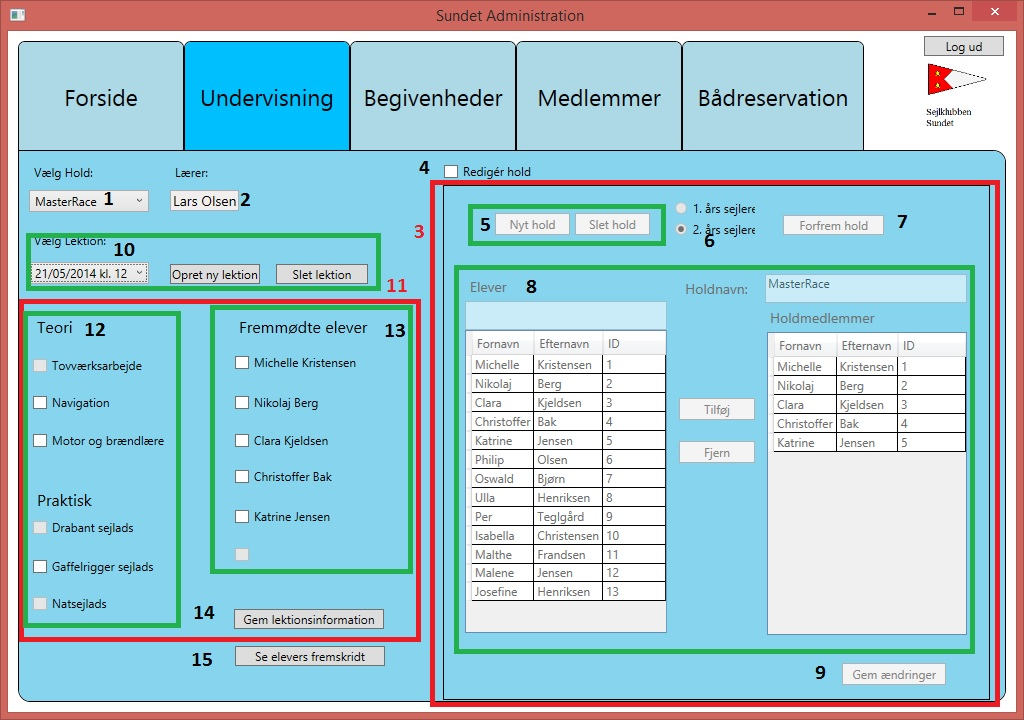
\includegraphics[width=1\textwidth]{images/UI/StudyTeacherMarked.jpg}
  \caption[UIStudyTeacher]{UI for undervisning tab som underviser og admin, markeringer bruges til forklaringer nedenfor}
  \label{fig:StudyTeacher}
\end{figure}

På \myref{fig:StudyTeacher} ses en 'usercontrol' for 'StudyTeacher'. På de markerede områder ses grupperinger af brugergrænsefladens funktioner, som er sammenhængende.
\textbf{1} referere til en 'combobox', som benyttes til valg af hold. 
Denne 'combobox' har indflydelse på det meste af undervisningsdelen, da denne information er afhængig af hvilket hold, som er valgt.
\textbf{2} henviser til en 'checkbox', som har kontrol over \textbf{3}, et 'grid' indeholdende funktionalitet til brug af redigering samt kreation af hold.
\textbf{4} er tilføjelse og sletning af hold, ``Slet hold'' knappen sletter det hold, som er valgt i \textbf{1}, mens ``Nyt hold'' knappen åbner et 'nested window', 'NewTeam', i programmet, hvor et nyt hold kan blive oprettet.
\textbf{5} disse 'radio buttons' benyttes for at vælge om holdet er 1. års eller 2. års sejlere.
\textbf{6} dette område benyttes til at tilføj og fjerne medlemmer ved brug af ``Tilføj'' og ``Fjern'' knapperne. 
Det venstre 'datagrid' benyttes til søgning af medlemmer. I dette grid kan alle 'StudentMember' findes, mens i det højre 'datagrid' ses de studerende, som der er på det valgte hold i \textbf{1}.
\textbf{7} denne knap gemmer ændringer for holdet. Dette er lavet separat for at undgå kommunikation med database ved hvert klik.
\textbf{8} denne knap angiver et duelighedsbevis til de medlemmer på det valgte hold i \textbf{1}, som opfylder alle undervisningskrav.
\textbf{9} referer til et grid med lektionsinformation. Hvis der ikke er valgt en lektion i \textbf{13}, er dette 'grid' ikke muligt at benytte.
\textbf{10} denne række af 'checkboxe' bruges til at krydse af hvad der er blevet undervist i på den valgte lektion og \textbf{11} benyttes ligeledes til at afkrydse hvilke elever var til stede.
\textbf{12} fungerer for lektion ligesom \textbf{7} for hold og er lavet til samme formål.
\textbf{13} er en 'combobox' som bruges til valg af lektion.
Den sidste funktion \textbf{14} åbner et nyt 'window', 'NewLecture', hvor man kan oprette en ny lektion for det givne hold valgt i \textbf{1}.

\paragraph{StudyStudent}

\begin{figure}[htbp]
  \centering
  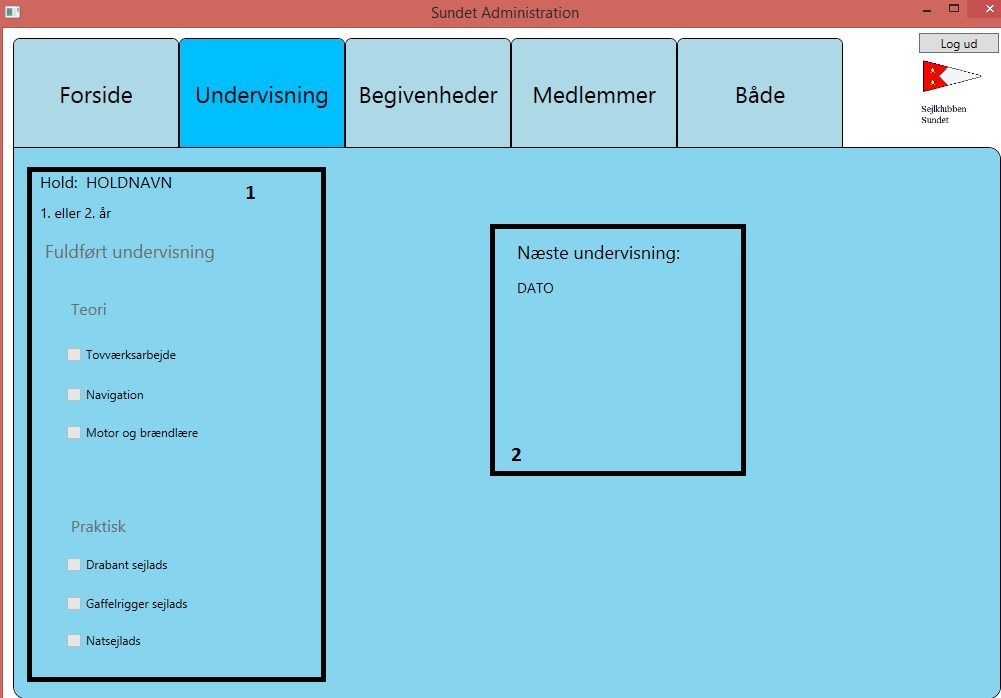
\includegraphics[width=1\textwidth]{images/UI/StudyStudentMarked.jpg}
  \caption[UIStudyStudent]{UI for undervisning tab som student, markeringer bruges til forklaringer nedenfor}
  \label{fig:StudyStudent}
\end{figure}

På \myref{fig:StudyStudent} ses en 'usercontrol' for 'StudyStudent'. \textbf{1} indeholder information omkring personens undervisning, 'checkbox'ene' indikerer undervisningsområder for den student som er logget ind, mens teksten ovenfor viser hvilket hold personen er på. \textbf{2} viser den næste lektionstidspunkt for det hold, studenten er tilknyttet.

\paragraph{NewLecture og NewTeam}

\begin{figure}[htbp]
\centering
\begin{minipage}{.5\textwidth}
  \centering
  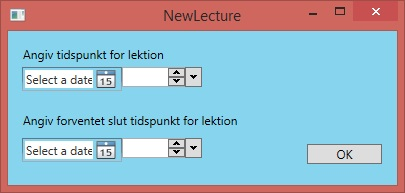
\includegraphics[width=0.8\textwidth]{images/UI/NewLecture.jpg}
  \caption[UINewLecture]{UI for NewLecture window}
  \label{fig:NewLecture}
\end{minipage}%
\begin{minipage}{.5\textwidth}
  \centering
  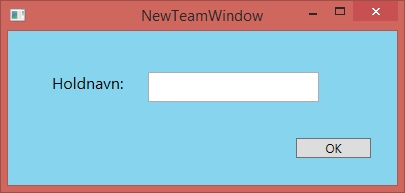
\includegraphics[width=0.8\textwidth]{images/UI/NewTeam.jpg}
  \caption[UINewTeam]{UI for NewTeam window}
  \label{fig:NewTeam}
\end{minipage}%
\end{figure}

På \myref{fig:NewLecture} ses et 'window' for 'NewLecture'. 
I 'NewLecture' vælges der to datoer ud i fremtiden. Disse bruges til at oprette en lektion, hvilket sker når der trykkes 'OK'. 
På \myref{fig:NewTeam} ses 'NewTeam'. Her skrives et holdnavn i tekstboksen, og således kan et hold oprettes.

\subsubsection{Code-Behind}
\paragraph{StudyTeacher}
\paragraph{StudyStudent}
\paragraph{NewLecture}
'NewLecture' er for brugeren simpel at benytte, der er dog mere funktionalitet i dette vindue end der bliver vist for brugeren.\fxnote{Menes der almindelig bruger set i forhold til administrator?}

\begin{lstlisting}[caption={Kode for 'OK' knap i 'NewLecture' 'Window'.}\label{NewLectOk}]
private void CompleteLectureCreate_Click(object sender, RoutedEventArgs e)
        {
            var lecture = new Lecture
            {
                DateOfLecture = DateTimePickerPlannedLectureTime.Value
            };
            DalLocator.LectureDal.Create(lecture);
            var Departure = DateTimePickerPlannedLectureTime.Value;
            var Arrival = DateTimePickerPlannedLectureTimeEnd.Value;
            var book = new CreateBoatBookingWindow(Departure, Arrival, _currentTeam);
        }
\end{lstlisting}
I \myref{NewLectOk} ses koden for ``OK'' knappen i 'NewLecture' vinduet. Datetimepicker bliver aflæst og informationen brugt til at oprette en 'Lecture'. Yderligere bliver informationen også gemt i henholdsvis 'Departure' og 'Arrival'. Disse bliver videresendt i en constructer for booking af både, 'CreateBoatBookingWindow()'. Dette er ``OK'' knappens indirekte funktionalitet. Funktionaliteten af dette kan ses på \myref{IndirekteBook}.

\begin{lstlisting}[caption={Dette kode bliver indirekte udført når der trykkes på 'OK' knappen, og opretter en bådreservation for lektionen.}\label{IndirekteBook}]
public CreateBoatBookingWindow(DateTime departure, DateTime arrival, Team currentTeam) 
	   : this(-1)
        {
            List<Boat> boats = new List<Boat>();
            boats = DalLocator.BoatDal.GetAll().ToList();
            Boat Anya = new Boat
            {
                Type = (currentTeam.Level == Team.ClassLevel.Second) ? BoatType.Gaffelrigger 
                : BoatType.Drabant
            };

            Boat currentBoat = boats.FirstOrDefault(
                x => x.Type == Anya.Type);

            BoatComboBox.SelectedIndex = boats.FindIndex(b => b == currentBoat);
            CrewList.Add(GlobalInformation.CurrentUser);
            CaptainComboBox.SelectedIndex = 0;
            foreach (var member in currentTeam.TeamMembers)
            {
                CrewList.Add(member);
            }
            DateTimeStart.Value = departure;
            DateTimeEnd.Value = arrival;
            PurposeTextBox.Text = "Undervisning af:" + currentTeam.Name;
            SaveButton_Click(new object(), new RoutedEventArgs());
        }
\end{lstlisting}
Denne constructer nedarver fra 'CreateBoatBookingWindow()' constructeren, som tager en paramter, index. Hertil benyttes ': this(-1)', ses på linje 2, for at sætte combobox'en, der styrer valg af booking, kan ses på <indsæt reference til BoatBooking>\fxnote{look at <>}, til null.\fxnote{Dårlige sætninger imo}
Alt efter om sejlerholdet er et 1. eller 2. års-hold, skal der bookes henholdsvis en drabant eller en gaffelrigger. Dette håndteres på linje 6 - 15. Der laves en lokal båd, Anya, hvis 'BoatType' bliver sat gennem en 'conditional operator'.
Herefter benyttes et 'lambda expression' til at finde den første båd af den korrekte type i databasen og 'boatcombobox', som styrer valg af båd, bliver sat til denne.
Efterfølgende bliver den administrator eller underviser der opretter lektionen sat som kaptajn. Det medsendte hold tilføjes 'CrewList', Departure og Arrival sættes også til de medsendte værdier. Formål bliver sat til undervisning og til sidst kaldes det event, som fuldfører bookningen.\fxnote{Enten slettes alle de apostroffer omkring de udvalgte navneord eller tilføjes til alle andre specielle navneord, fra Undervisning og ned passer ikke rigtig sammen med det tidligere skrevet}

